\section{Problems}

\begin{questions}
\question{Solve the Huggett economy}
\begin{solution}

Here is a link to my code: \url{https://github.com/filipmellgren/QMM/tree/main/ps2}

\begin{itemize}
	\item The grid points for income are \verbatiminput{income_states.txt}
	\item The equilibrium interest rate is \verbatiminput{root_rate.txt}
	\item 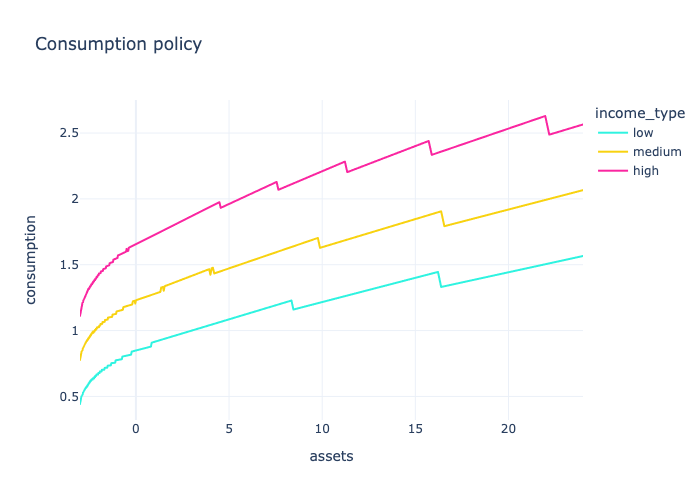
\includegraphics[scale=0.5]{figures/consumption_by_income.png}
\end{itemize}

Solution values come very close to 0. I think there might still be some issues with the ergodic distribution. Either I coded something wrong or there was a numeric drift because it didn't always sum to one, so I scaled it after each iteration.

For fun, here is a plot showing time to convergence as a function of the number of gridpoints in the asset and action dimensions:

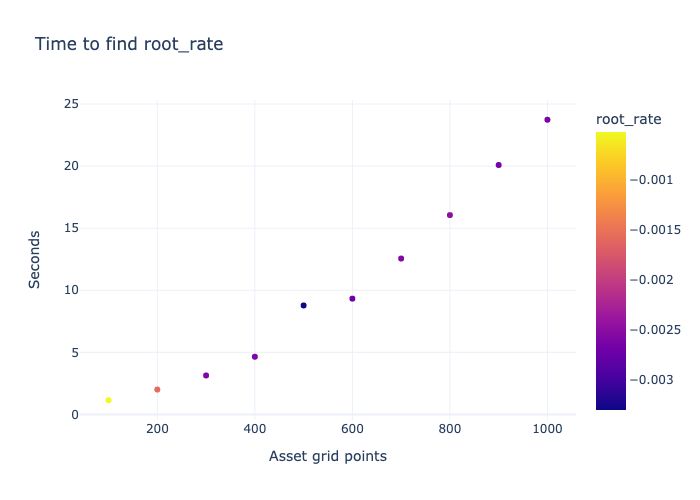
\includegraphics[scale=0.5]{figures/time_to_converge.png}

I solved this assignment using the Numpy and Numba packages in Python.

The policy matrix looks as follow:

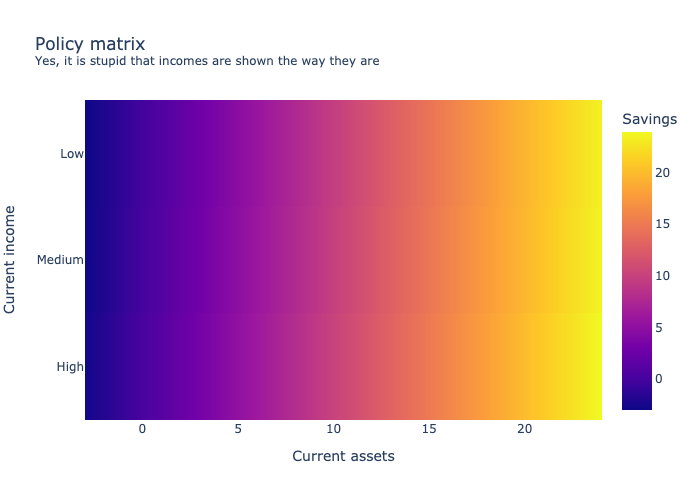
\includegraphics[scale=0.5]{figures/policy_matrix.png}


\end{solution}
\question{Solve the Huggett economy}
Money doesn't earn interest, therefore $r = 1$.

\begin{solution}
	\begin{itemize}
		\item In an economy with a zero yielding asset in stationary equilibrium, meaning prices are constant. If the true solution has a positive interest rate, then nobody would demand money unless they cost negative number of goods (?). If the true solution has a negative interest rate, then everybody demands money up to the borrowing constraint so the price of goods in terms of money is 10/3.
		\item Prices of goods in terms of money increases by factor 10.
		\item Effect of introducing money into the Huggett economy: it depends on whether the market clearing interest rate is positive or negative. With a negative rate, people would want to hold money and they become valuable. With a positive rate, they are irrelevant as people will want the asset instead at that rate. 
		\item The new equilibrium interest rate is \verbatiminput{new_root_rate.txt}. Which is higher than before. Although I guess it should really be lower because a higher risk makes individuals want to insure more by holding assets, so at the previous rate people would want too much insurance to compensate for the higher income risk. To clear the market, the price of insuring must therefore increase which means it returns less.
	\end{itemize}
\end{solution}


\end{questions}




